\documentclass[tikz,border=14pt]{standalone}
\usetikzlibrary{arrows.meta,positioning}
\begin{document}
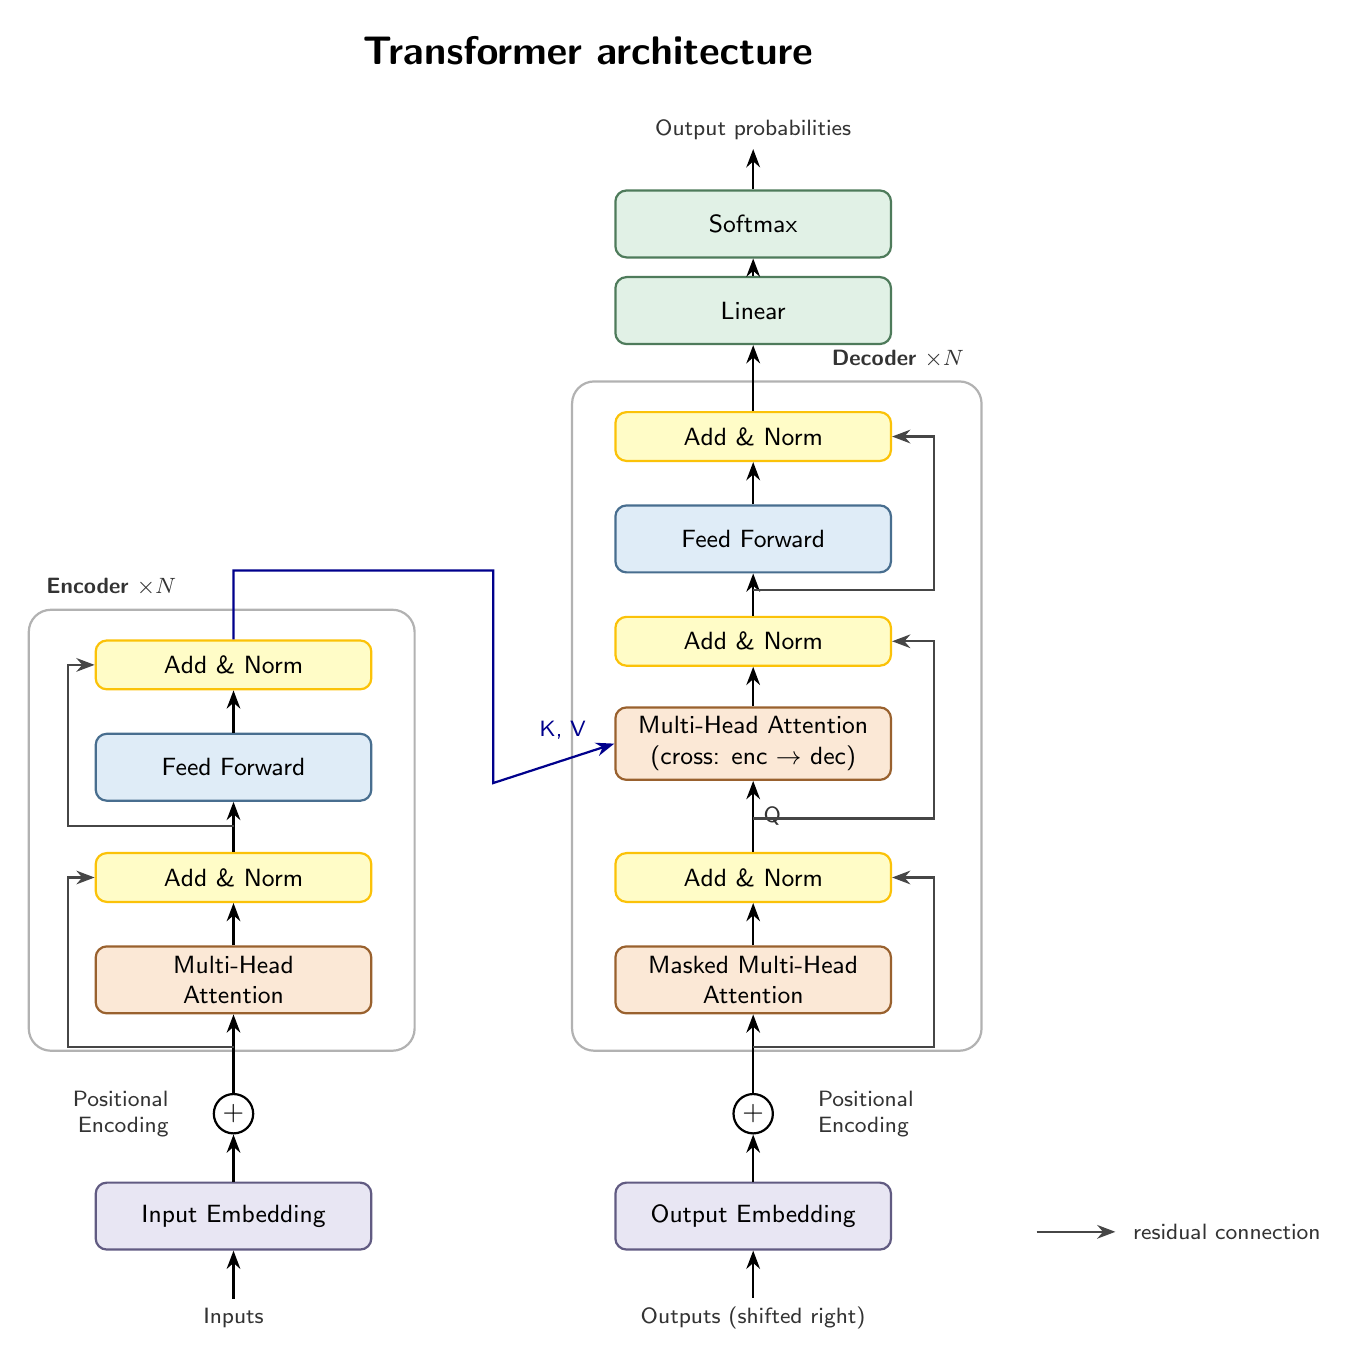
\begin{tikzpicture}[
  >=Stealth,
  font=\sffamily,
  blk/.style={draw=#1!65!black,fill=#1!22,rounded corners=4pt,
    minimum width=3.5cm,minimum height=0.85cm,align=center,thick,font=\small\sffamily},
  addnorm/.style={draw=yellow!55!orange,fill=yellow!22,rounded corners=4pt,
    minimum width=3.5cm,minimum height=0.62cm,align=center,thick,font=\small\sffamily},
  plus/.style={draw=black,circle,minimum size=0.5cm,inner sep=0pt,thick,fill=white},
  sig/.style={->,thick},
  res/.style={->,thick,gray!55!black},
  lab/.style={font=\footnotesize\sffamily,text=gray!40!black}]

  \definecolor{attnc}{RGB}{235,150,70}
  \definecolor{ffc}{RGB}{110,170,220}
  \definecolor{embc}{RGB}{150,140,200}
  \definecolor{linc}{RGB}{120,190,140}

  % ================= encoder column (x=0) =================
  \node[lab] (inp) at (0,-0.9) {Inputs};
  \node[blk=embc] (emb) at (0,0.4) {Input Embedding};
  \node[plus] (pe1) at (0,1.7) {$+$};
  \node[lab,anchor=east,align=right] at (-0.7,1.7) {Positional\\Encoding};
  \node[blk=attnc] (mha) at (0,3.4) {Multi-Head\\Attention};
  \node[addnorm] (an1) at (0,4.7) {Add \& Norm};
  \node[blk=ffc] (ff) at (0,6.1) {Feed Forward};
  \node[addnorm] (an2) at (0,7.4) {Add \& Norm};

  % encoder frame
  \draw[gray!60,thick,rounded corners=8pt] (-2.6,2.5) rectangle (2.3,8.1);
  \node[lab,anchor=south west] at (-2.5,8.15) {\textbf{Encoder} $\times N$};

  % encoder signal path
  \draw[sig] (inp) -- (emb);
  \draw[sig] (emb) -- (pe1);
  \draw[sig] (pe1) -- (mha);
  \draw[sig] (mha) -- (an1);
  \draw[sig] (an1) -- (ff);
  \draw[sig] (ff) -- (an2);

  % encoder residuals (left side)
  \draw[res] (0,2.55) -- (-2.1,2.55) -- (-2.1,4.7) -- (an1.west);
  \draw[res] (0,5.35) -- (-2.1,5.35) -- (-2.1,7.4) -- (an2.west);

  % ================= decoder column (x=6.6) =================
  \node[lab] (outp) at (6.6,-0.9) {Outputs (shifted right)};
  \node[blk=embc] (emb2) at (6.6,0.4) {Output Embedding};
  \node[plus] (pe2) at (6.6,1.7) {$+$};
  \node[lab,anchor=west,align=left] at (7.3,1.7) {Positional\\Encoding};
  \node[blk=attnc] (mmha) at (6.6,3.4) {Masked Multi-Head\\Attention};
  \node[addnorm] (an3) at (6.6,4.7) {Add \& Norm};
  \node[blk=attnc] (xatt) at (6.6,6.4) {Multi-Head Attention\\(cross: enc $\to$ dec)};
  \node[addnorm] (an4) at (6.6,7.7) {Add \& Norm};
  \node[blk=ffc] (ff2) at (6.6,9.0) {Feed Forward};
  \node[addnorm] (an5) at (6.6,10.3) {Add \& Norm};

  % decoder frame
  \draw[gray!60,thick,rounded corners=8pt] (4.3,2.5) rectangle (9.5,11.0);
  \node[lab,anchor=south east] at (9.4,11.05) {\textbf{Decoder} $\times N$};

  % decoder head
  \node[blk=linc] (lin) at (6.6,11.9) {Linear};
  \node[blk=linc] (smx) at (6.6,13.0) {Softmax};
  \node[lab] (prob) at (6.6,14.2) {Output probabilities};

  % decoder signal path
  \draw[sig] (outp) -- (emb2);
  \draw[sig] (emb2) -- (pe2);
  \draw[sig] (pe2) -- (mmha);
  \draw[sig] (mmha) -- (an3);
  \draw[sig] (an3) -- (xatt) node[lab,midway,right] {Q};
  \draw[sig] (xatt) -- (an4);
  \draw[sig] (an4) -- (ff2);
  \draw[sig] (ff2) -- (an5);
  \draw[sig] (an5) -- (lin);
  \draw[sig] (lin) -- (smx);
  \draw[sig] (smx) -- (prob);

  % decoder residuals (right side)
  \draw[res] (6.6,2.55) -- (8.9,2.55) -- (8.9,4.7) -- (an3.east);
  \draw[res] (6.6,5.45) -- (8.9,5.45) -- (8.9,7.7) -- (an4.east);
  \draw[res] (6.6,8.35) -- (8.9,8.35) -- (8.9,10.3) -- (an5.east);

  % encoder output to cross-attention (K, V)
  \draw[sig,blue!55!black] (an2.north) -- (0,8.6) -- (3.3,8.6) -- (3.3,5.9)
    -- (xatt.west) node[lab,pos=0.85,above left,text=blue!55!black] {K, V};

  % residual legend
  \draw[res] (10.2,0.2) -- (11.2,0.2);
  \node[lab,anchor=west] at (11.3,0.2) {residual connection};

  % title
  \node[font=\sffamily\bfseries\Large] at (4.5,15.2) {Transformer architecture};
\end{tikzpicture}
\end{document}
